\section{Punto de Vista de Uso de Aplicación}

El punto de vista del uso de la aplicación describe cómo se usan las aplicaciones para admitir uno o más procesos comerciales y cómo las usan otras aplicaciones. Se puede utilizar para diseñar una aplicación identificando los servicios que necesitan los procesos de negocio y otras aplicaciones, o para diseñar procesos de negocio al describir los servicios que están disponibles. Además, dado que identifica las dependencias de los procesos comerciales con las aplicaciones, puede ser útil para los gerentes operativos responsables de estos procesos.


\subsection{Modelo de Uso de Aplicación}
\begin{figure}[h!]
	\centering
	\includegraphics[width=.8\linewidth]{imgs/modelo/UsoAplicacion}
	\caption{Modelo Uso de Aplicación}
\end{figure}

El punto de vista de Uso de aplicación es la interconexión entre la capa de negocio y la de aplicación, iniciando desde el proceso llegando hasta el componente por medio de la interfaz y el servicio que brinda este componente en el proceso mencionado. Las demás características de este punto de vista son: de la parte de negocio está el evento, el objeto, el actor, la colaboración y finalmente el proceoo que se conecta con el servicio de la capa de aplicación y llega finalmente al componente por medio de la interfaz y el objeto.

\newpage

\subsection{Caso  de Uso de Aplicación}
\begin{figure}[h!]
	\centering
	\includegraphics[width=.8\linewidth]{imgs/caso/aplicacion/UsoAplicacion}
	\caption{Caso Uso de Aplicación}
\end{figure}

En el caso del proyecto "Tu Perfil", se encuentra como proceso principal el acompañamiento vocacional, y para este proceso se encuentran tres componentes estrechamente relacionados y se realiza la conexión entre estos componentes y el proceso por medio del servicio que brindan, el primer componente es el de contexto, el cual brinda el servicio de la escogencia de juego; el segundo componente es el de juego, el cual brinda el servicio de jugar y finalmente, el tercer componente es el perfilamiento con el servicio del direccionamiento según la vocación.

\newpage